%%%%%%%%%%%%%%%%%%%%%%%%%%%%%%%%%%%%%%%%%%%%%%%%%%%%%%%%%%%%%%%%%%%%%%%%%%
% Voltage-mode control loop (Exercise 12, Tasks 1 to 3)
%%%%%%%%%%%%%%%%%%%%%%%%%%%%%%%%%%%%%%%%%%%%%%%%%%%%%%%%%%%%%%%%%%%%%%%%%%

\begin{figure}[htb]
	\begin{center}
		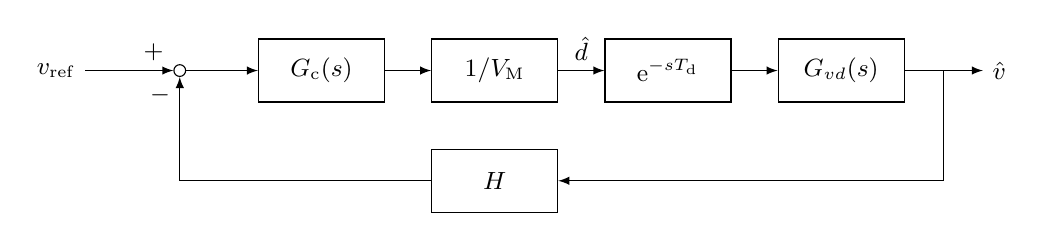
\begin{tikzpicture}[font=\small, >=latex, box/.style={draw, minimum width=1.6cm, minimum height=0.8cm, align=center}]
			\node[draw, circle, inner sep=1.5pt] (sum) at (0,0) {};
			\node[box] (gc) at (1.8,0) {$G_\mathrm{c}(s)$};
			\node[box] (pwm) at (4.0,0) {$1/V_\mathrm{M}$};
			\node[box] (del) at (6.2,0) {$\mathrm{e}^{-sT_\mathrm{d}}$};
			\node[box] (gvd) at (8.4,0) {$G_{vd}(s)$};
			\node[box] (h) at (4.0,-1.4) {$H$};
			\draw[->] (-1.2,0) node[left]{$v_\mathrm{ref}$} -- (sum.west) node[above left]{$+$};
			\draw[->] (sum) -- (gc); \draw[->] (gc) -- (pwm); \draw[->] (pwm) -- node[above]{$\hat{d}$} (del); \draw[->] (del) -- (gvd);
			\draw[->] (gvd) -- (10.2,0) node[right]{$\hat{v}$};
			\draw[->] (9.7,0) |- (h.east); \draw[->] (h.west) -| (sum.south) node[below left]{$-$};
		\end{tikzpicture}
	\end{center}
	\caption{Voltage-mode loop with modulator gain $1/V_\mathrm{M}$, total delay $T_\mathrm{d}$ and sensor gain $H$; loop gain $T=HG_\mathrm{c}G_{vd}\mathrm{e}^{-sT_\mathrm{d}}/V_\mathrm{M}$}
	\label{fig:ex12_loop}
\end{figure}
